\documentclass[12pt,a4paper]{article}
\usepackage[utf8]{inputenc}
\usepackage[czech, english]{babel}
\usepackage[T1]{fontenc}
\usepackage{amsmath}
\usepackage{amsfonts}
\usepackage{amssymb}
\usepackage{graphicx}
\usepackage[final,pdftex, colorlinks=false]{hyperref}
\usepackage{xcolor}
\usepackage{comment}
\usepackage{todonotes}
\usepackage{floatrow}
\usepackage{multirow}
\usepackage{algorithm}
\usepackage{algorithmicx}
\usepackage{algpseudocode}
\usepackage{titletoc}
\usepackage{pdfpages}
\usepackage{hhline}
\usepackage{makecell}

\usepackage{listings}			%vkladani kodu
\lstset{basicstyle=\ttfamily,
  showstringspaces=false,
  commentstyle=\color{red},
  keywordstyle=\color{blue},
  breaklines=true,
  frame=lines,
}

%okraje
\usepackage[
left=35mm,
right=25mm,
top=40mm,
bottom=35mm]
{geometry}

\author{Adam Laža}

%%%%%%%%%%Prikazy%%%%%%%%%%
\renewcommand\baselinestretch{1.3}		%radkovani
\parskip=0.8ex plus 0.4ex minus 0.1 ex	%mezera mezi odstavci

\newcommand{\keywords}[2]{\noindent\textbf{#1: }#2}
\newcommand{\necislovana}[1]{%
\phantomsection
\addcontentsline{toc}{section}{#1}

%\newcommand{\exedout}{%
%  \rule{0.8\textwidth}{0.5\textwidth}%
%}


\section*{#1}
\markboth{\uppercase{#1}}{}
}
%%%%%%%%%%%%%%%%%%%%%%%%%%%%

%%%%%%%%%%Zahlavi%%%%%%%%%%%
\usepackage{fancyhdr}
\fancyhead[L]{CTU in~Prague}
\setlength{\headheight}{16pt}
%%%%%%%%%%%%%%%%%%%%%%%%%%%%

\begin{document}
\pagestyle{empty}

\newpage
\begin{center}
%napisy
\newcommand{\napisCVUT}{Czech technical university in Prague}
\newcommand{\napisFS}{Faculty of Civil engineering}
\newcommand{\napisProgram}{Study programme Geodesy and cartography}
\newcommand{\napisObor}{Geomatics}
\newcommand{\napisKatedra}{Department of geomatics}
\newcommand{\napisVedouci}{Supervisor: Ing. Martin Landa, Ph.D.}
\newcommand{\napisAutor}{Bc. Adam Laža}
\newcommand{\napisDatum}{Prague 2018}
\newcommand{\napisNazevI}{Process isolation in PyWPS framework}
\newcommand{\napisNazevAjI}{Izolace procesů ve frameworku PyWPS}
\newcommand{\napisDiplomka}{Master thesis}
\newcommand{\napisPraha}{Prague 2018}
%
% prikazy
%\newcommand{\velka}[1]{\uppercase{#1}}
\newcommand{\velka}[1]{\textsc{#1}}
%
% 
\newif\ifpatitul
\patitultrue

\ifpatitul
{\Large\velka{\napisCVUT}}\\
\velka{\Large\napisFS}\\
\vfill
{\LARGE\velka{\napisDiplomka}}
\vfill
{\large\napisPraha\hfill\napisAutor}
\newpage
\fi%patitul


{\Large\velka{\napisCVUT}}\\
{\Large\velka{\napisFS}}\\
{\Large\velka{\napisProgram}}\\
{\Large\velka{\napisObor}}
\vfill

\includegraphics[width=3cm]{logo_cvut_cb} %~
\vfill
{\Large\velka{\napisDiplomka}}\\
\Large\velka{\napisNazevI}\\
\large\velka{\napisNazevAjI}
\vfill
{\large%
\napisVedouci\\
\napisKatedra\\
\bigskip
\napisDatum\hfill\napisAutor}
\end{center}


%\newpage
%\includepdf[pages={1}]{../formulare/zadani.pdf}

\newpage

\selectlanguage{english}
\begin{abstract}
\bigskip
This master thesis is dedicated to isolation of PyWPS processes as one of the OGC WPS implementation. OGC WPS is Web Processing Service
Standard defined by Open Geospatial Consorcium. The practical part contains an introductory research where various solutions how 
to reach the process isolation are considered and described. Based on the research the Docker technology has been chosen for the 
implementation of process isolation.  In the theoretical part Docker technology is described as well as the OGC WPS standard and 
its PyWPS implementation written in Python.

\bigskip
\keywords{Keywords}
OGC WPS, PyWPS, Docker container, Python, process izolation, Web Processing Service.
\end{abstract}

\selectlanguage{czech}
\begin{abstract}
\bigskip
\todo[inline]{Překlad WPS - Webová Procesingová??? Služba, OG??}
Tato diplomová práce se věnuje možnostem izolace procesů v rámci frameworku PyWPS jako jedné z implementací OGC WPS. Webová Procesingová 
Služba je standard vydaný a dále rozšiřovaný Open Geospatial Consorciem. Praktická část obsahuje úvodní rešerši, ve které jsou popsány
různé možnosti, jak izolace jednotlivých procesů dosáhnout. Na základě rešerše byla pro implementaci vybraná technologie Docker.
V teoretické části je popsána jak technologie Docker, tak OGC WPS standard a jeho implementace PyWPS napsaná v jazyce Python.

\bigskip
\keywords{Klíčová slova}
OGC WPS, PyWPS, Docker kontejner, Python, izolace procesu, Webová Procesingová Služba.
\end{abstract}

\selectlanguage{english}
%%%%Prohlaseni a podekovani
\newcommand{\odsaditodzhora}{\hskip1pt\vfill}
\newpage
\odsaditodzhora
\noindent {\bf Declaration of authorship}
I declare that the work presented here is, to the best of my knowledge and
belief, original and the result of my own investigations, except as acknowledged.
Formulations and ideas taken from other sources are cited as such


\begin{flushleft}
\begin{tabular}{cp{0.3\textwidth}c}
In Prague .................
& 
&
..................................
\\
&&
(author sign)
\end{tabular}

\end{flushleft}
\newpage

\odsaditodzhora
\noindent {\bf Acknowledgement}

\todo[inline]{Podekovani}

\newpage
\tableofcontents

\newpage
\pagestyle{fancy}

\necislovana{Introduction} 
Mame hromadu dat, ktere je potreba zpracovat. Hodne to ulehci, kdyz to budem moct nejak standardizovat a pak pouzivat na cloudu.

https://pdfs.semanticscholar.org/bb17/7b12791d5ea58811955555be2d48226fd5ae.pdf
\todo[inline]{Uvod}

\newpage
\part{Technological background}

\newpage
\section{Web Processing Service}

\subsection{History}
First mention of the Web Processing Service was in October 2004. Back then it
was named Geoprocessing Service \cite{OGC_news}. The specification was first 
implemented as a prototype in 2004 by Agriculture and Agri-Food Canada (AAFC).
In its further development during a Geoprocessing Services Interoperability Experiment \cite{WPS_experiment} 
the name was changed to "Web Processing Service" to avoid the acronym GPS, since 
this would have caused confusion with the conventional use of this acronym for 
Global Positioning System \cite{WPS_standart_1.0}. The first version of WPS was released in
September 2005 \cite{WPS_first}. The experiment demonstrated that various clients
could easily access and bind to services which were set up according the WPS Implementation
specification.

Currently two major versions of WPS Standard exist. The WPS version 1.0.0 is currently used mostly.
If not explicitly said this thesis is dedicated to the version 1.0.0. The WPS version 2.0.0 was
released in 2015 \cite{WPS_second}.

\bigskip
\subsection{Web Processing Service}
The OpenGIS® Web Processing Service (WPS) Interface Standard defines a standardized interface
that facilitates the publishing of geospatil processes. Also provides rules how to standardize
requests and responses for geospatial processing services. 

\textit{Process} means any operation on spatial
data from simple ones as maps overlay or buffering to highly complex as complicated global models. Any kind of GIS 
funcionality can be offered to clients across network with correctly configured WPS. 

\textit{Publishing} means
creating human-readable metadata that allow user to discover and use service as well as making 
available machine-readable binding information.

\textit{Data} can be both vector or raster data and can be delivered across the network or be available
at the server.

The interface does not specify any specific processes that can be implemented by a WPS nor any specific
data inputs or outputs. instead it specifies a generic mechanisms to describe any geospatial process and
data required and produced by the process. The interface does not only provide mechanisms for calculation
but also to identify required data, initiate the calculation and manage output data so clients can access it. 

\bigskip
Web Processing Service as one of the OGC web services scpecifies three types of requests which can be requested
by a client and performed by a WPS server. The implementation of these three requests is mandatory by by all servers:
\begin{itemize}
\item{GetCapabilities}
\item{DescribeProcess}
\item{Execute}
\end{itemize}

\textit{GetCapabilities} - The request returns to client a Capabilities document that describes the abilities
of the specific server implementation. It also returns the name and abstract of each of the processes that can
be run on a WPS instance.

\textit{DescribeProcess} - The request returns details about the processes offered by a WPS instance. Describes
required inputs and produces outputs and their allowable formats.

\textit{Execute} - The request allows a client to run a specified process with provided parameters and returns
produced outputs.

\begin{figure}[h!]
\centering
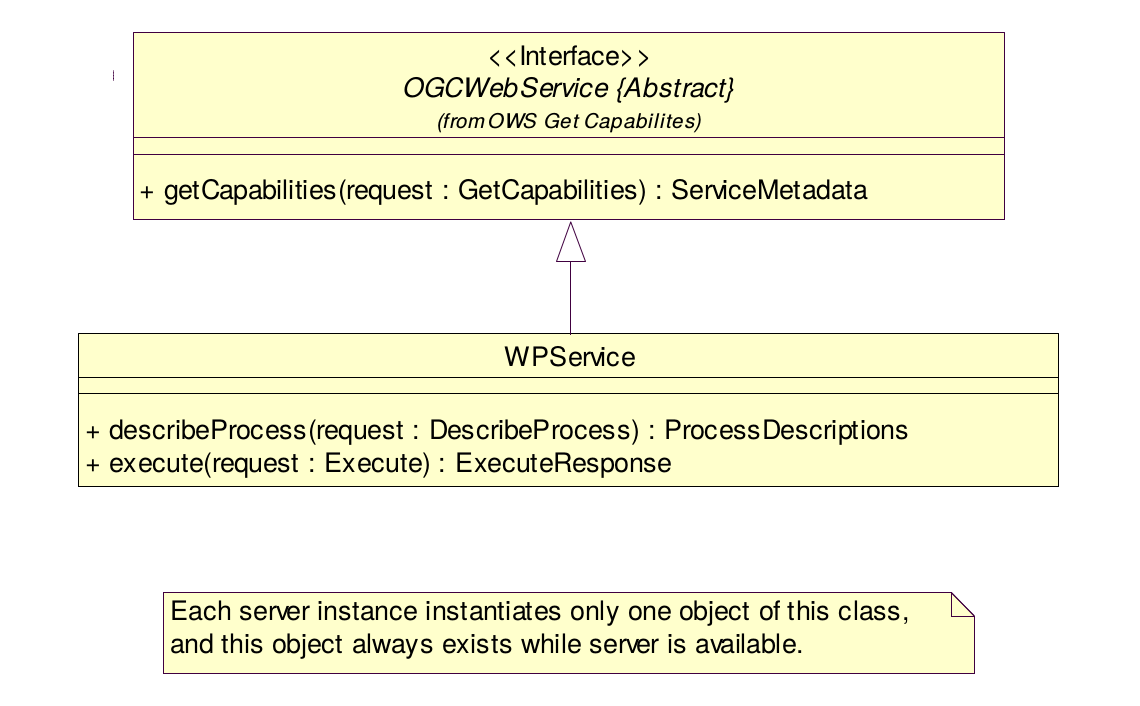
\includegraphics[width=0.78\textwidth]{img/WPS_class_diagram.png}
\caption{WPS interface UML description, source: \cite{WPS_standart_1.0}}
\label{fig:WPS_class_diagram}
\end{figure}

These operations are very similar to other OGC Web Services such as WMS, WFS, and WCS. Common interface aspects
are defined in the OpenGIS ® Web Services Common Implementation Specification \cite{OGC_common}. As seen at 
class diagram at Fig. \ref{fig:WPS_class_diagram} the WPS interface class inherits the GetCapabilities operation 
from OGCWebService interface class. The operations Execute and DescribeProcess are specific for the WPS. The WPS
operations are based on GET and POST requests.

\bigskip
\begin{table}[h!]
\catcode`\-=12
\centering
\begin{tabular}{|c|c|c|}
\hline
\multirow{2}{*}{Operation} & \multicolumn{2}{c|}{Request encoding} \\ \cline{2-3} 
                           & Mandatory          & Optional         \\ \hhline{|=|=|=|}
GetCapabilities            & KVP                & XML              \\ \hline
DescribeProcess            & KVP                & XML              \\ \hline
Execute                    & XML                & KVP              \\ \hline
\end{tabular}
\caption{Operations request encoding}
\label{tab:WPS_encoding}
\end{table}

The GetCapabilities and DescribeProcess shall use HTTP GET with KVP encoding and Execute operation shall use HTTP
POST with XML encoding. Summarized in Table \ref{tab:WPS_encoding}.

\bigskip
\subsubsection{GetCapabilities}
The GetCapabilities operation is mandatory. The operation allows clients to retrieve capabilities document (metadata)
from a server. The response XML document contains service metadata about server and all implemented processes description.

\todo[inline]{AcceptVersion vs version, AcceptFormats vs format}
\paragraph{GetCapabilities request}
\subparagraph{Request parameters}
\begin{table}[h!]
\catcode`\-=12
\centering
\begin{tabular}{|c|c|c|}
\hline
\thead{Name}               & \thead{Optionality and use} & \thead{Definition and format}    		\\ \hhline{|=|=|=|}
service=WPS                & Mandatory           & Service type identifier text 	\\ \hline
request=GetCapabilities    & Mandatory           & Operation name text              \\ \hline
AcceptVersion=1.0.0        & Optional            & Specification version            \\ \hline
Sections=All               & Optional            & \makecell{Comma-separated \\unordered list of sections} \\ \hline
updateSequence=XXX         & Optional            & \makecell{Service metadata \\document version}            \\ \hline
AcceptFormats=text/xml     & Optional            & \makecell{Comma-separated \\prioritized sequence of \\response formats} \\ \hline
\end{tabular}
\caption{GetCapabilities operation request URL parameters, source: \cite{OGC_common}}
\label{tab:WPS_GetCapabilities}
\end{table}

\begin{itemize}
\item\textit{service} - Mandatory parameter, WPS is only possible value.
\item\textit{request} - Mandatory parameter, GetCapabilities is only possible value.
\item\textit{version} - Optional parameter, version number. Three non-negative integers separated by decimal point. Servers and
their clients should support at least one defined version.
\item\textit{sections} - Optional parameter that contains a list of section names. Possible values are: \textit{ServiceIdentification,
ServiceProvider, OperationsMetadata, Contents, All}.
\item\textit{updateSequence} - Optional parameter for maintaining the consistency of a client cache of the contents of a service
metadata document. The parameter value can be an integer, a timestamp, or any other number or string.
\item\textit{updateSequence} - Optional parameter for maintaining the consistency of a client cache of the contents of a service
metadata document. The parameter value can be an integer, a timestamp, or any other number or string.
\item\textit{format} - Optional parameter that defines response format.
\end{itemize}

The GetCapabilities operation can be requested with parameters from table \ref{tab:WPS_GetCapabilities}. A corresponding
request URL looks like:
\url{http://localhost:5000/wps?service=WPS&request=GetCapabilities&Accept
Version=1.0.0&Section=ServiceIdentification,OperationsMetadata&update
Sequence=XXX&AcceptFormats=text/xml}

\bigskip
\paragraph{GetCapabilities response}
\subparagraph{Normal response}
When GetCapabilities operation requested a client retrieve service metadata document that contains sections specified in
\textit{sections} parameter. If the parameter value is \textit{All} or is not specified all sections retrieved.

\begin{itemize}
\item\textit{ServiceIdentification} - Server metadata.
\item\textit{ServiceProvider} - Server operating organization metadata.
\item\textit{OperationsMetadata} - Metadata about operations implemented by the WPS server, including URLs to request them.
\item\textit{ProcessOfferings} - List of processes with name and brief description implemented by the WPS server.
\end{itemize}
In addition to sections each GetCapabilities response should contains:
\begin{itemize}
\item\textit{version} - Specification version for GetCapabilities operation.
\item\textit{updateSequence} - Server metadata document version, value is increased whenever any change is made in complete service metadata document.
\end{itemize}

\subparagraph{GetCapabilities exceptions}
In case that WPS server encounters an error a client retrieve an exception report message with one of there exception code:

\begin{itemize}
\item\textit{MissingParameterValue} - GetCapabilities request does not contain a required parameter value.
\item\textit{InvalidParameterValue} - GetCapabilities request contains an invalid parameter value.
\item\textit{VersionNegotiation} - Any version from AcceptVersions parameter list does not match any version supported by the WPS server.
\item\textit{InvalidUpdateSequence} - Value of updateSequence parameter is greater than current value of service metadata updateSequence number.
\item\textit{NoApplicableCode} - Other exceptions.
\end{itemize}

\bigskip
\subsubsection{DescribeProcess}
The DescribeProcess operation is mandatory. The operation allows clients to retrieve a detailed description about one or more
processes implemented by a WPS server. The detailed information describe both required inputs and produced outputs and allowed
format.

\paragraph{DescribeProcess request}
\subparagraph{Request parameters}

\begin{itemize}
\item\textit{service} - Mandatory parameter, WPS is only possible value.
\item\textit{request} - Mandatory parameter, DescribeProcess is only possible value.
\item\textit{version} - Mandatory parameter, version number. Three non-negative integers separated by decimal point. Servers and
their clients should support at least one defined version.
\item\textit{Identifier} - Optional parameter, list of process names separated by comma. Another possible value is \textit{all}.
\end{itemize}

\begin{table}[h!]
\catcode`\-=12
\centering
\begin{tabular}{|c|c|c|}
\hline
\thead{Name}               & \thead{Optionality} & \thead{Definition and format}    		\\ \hhline{|=|=|=|}
service=WPS                & Mandatory           & Service type identifier text 	\\ \hline
request=DescribeProcess    & Mandatory           & Operation name text              \\ \hline
version=1.0.0              & Mandatory           & WPS specification version            \\ \hline
Identifier=buffer          & Optional            & \makecell{List of one or more process\\ identifiers, separated by commas} \\ \hline
\end{tabular}
\caption{DescribeProcess operation request URL parameters, source: \cite{OGC_common}}
\label{tab:WPS_DescribeProcess}
\end{table}

The DescribeProcess operation can be requested with parameters from table \ref{tab:WPS_DescribeProcess}. A corresponding
request URL looks like: \url{http://localhost:5000/wps?request=DescribeProcess&service=WPS&identifier=all&version=1.0.0}

\paragraph{DescribeProcess response}
\subparagraph{Normal response}
Normal response to DescribeProcess request contains or more process descriptions for requested process identifiers in 
\textit{ProcessDescriptions} structure. Each
process description contains detailed information about process in \textit{ProcessDescription} including process inputs and outputs description. Number
of inputs or outputs is not limited. Three types of input or outpus exist:
\todo[inline]{Doplnit popisy dat}
\begin{itemize}
\item\textit{LiteralData} - 
\item\textit{ComplexData} - 
\item\textit{BoundingBoxData} - 
\end{itemize}


\begin{table}[h!]
\catcode`\-=12
\centering
\begin{tabular}{|c|c|c|}
\hline
\thead{Name}               & \thead{Optionality} & \thead{Definition and format}    		\\ \hhline{|=|=|=|}
ProcessDescription	       & Mandatory           & \makecell{Full description of process \\ including inputs/outputs}             \\ \hline
service=WPS                & Mandatory           & Service type identifier text 	\\ \hline
version=1.0.0              & Mandatory           & Operation specification version          \\ \hline
lang			           & Mandatory           & Language identifier \\ \hline
\end{tabular}
\caption{Parts of ProcessDescriptions data structure, source: \cite{WPS_standart_1.0}}
\label{tab:WPS_ProcessDescriptions}
\end{table}

\begin{table}[h!]
\catcode`\-=12
\centering
\begin{tabular}{|c|c|c|}
\hline
\thead{Name}               & \thead{Optionality} & \thead{Definition and format}    		\\ \hhline{|=|=|=|}
Identifier      	       & Mandatory           & Process identigier             \\ \hline
Title 			           & Mandatory           & Process title 				  \\ \hline
Abstract		           & Optional            & Brief description              \\ \hline
Metadata		           & Optional            & \makecell{Reference to more metadata \\about this process} \\ \hline
Profile			           & Optional            & \makecell{Profile to which the WPS \\process complies} \\ \hline
processVersion	           & Mandatory           & Release version of process \\ \hline
WSDL    		           & Optional            & \makecell{Location of a WSDL document \\that describes this process} \\ \hline
DataInputs		           & Optional            & \makecell{List of the required and \\optional inputs} \\ \hline
ProcessOutputs	           & Mandatory           & \makecell{List of the required and\\optional outputs} \\ \hline
storeSupported	           & Optional            & \makecell{Complex data outputs can be \\stored by WPS server} \\ \hline
statusSupported	           & Optional            & \makecell{Execute response can be returned\\ quickly with status information} \\ \hline
\end{tabular}
\caption{Parts of ProcessDescription data structure, source: \cite{WPS_standart_1.0}}
\label{tab:WPS_ProcessDescription}
\end{table}

\subparagraph{DescribeProcess exceptions}
In case that WPS server encounters an error a client retrieve an exception report message with one of there exception code:

\begin{itemize}
\item\textit{MissingParameterValue} - GetCapabilities request does not contain a required parameter value.
\item\textit{InvalidParameterValue} - GetCapabilities request contains an invalid parameter value.
\item\textit{NoApplicableCode} - Other exceptions.
\end{itemize}

\bigskip
\subsubsection{Execute}
The Execute operation is mandatory. The operation allows clients to run a specified process implemented by a server.
Inputs can be included directly in the request body or be referenced as web accesible resource. The outputs are returned
in XML response document, either directly embedded within the response document or stored as resource accesible by
returned URL.

Ussualy the response document is returned right after the process execution is completed. However it is possible to get
response document right after sending request. In this case, returned response document contains a URL link from which the
final response document can be retrieved after completed process execution. Client can request execution status update to
find out the amount of processing remaining if the execution is not completed. Shown at Fig. \ref{fig:WPS_activity}.

\begin{figure}[h!]
\centering
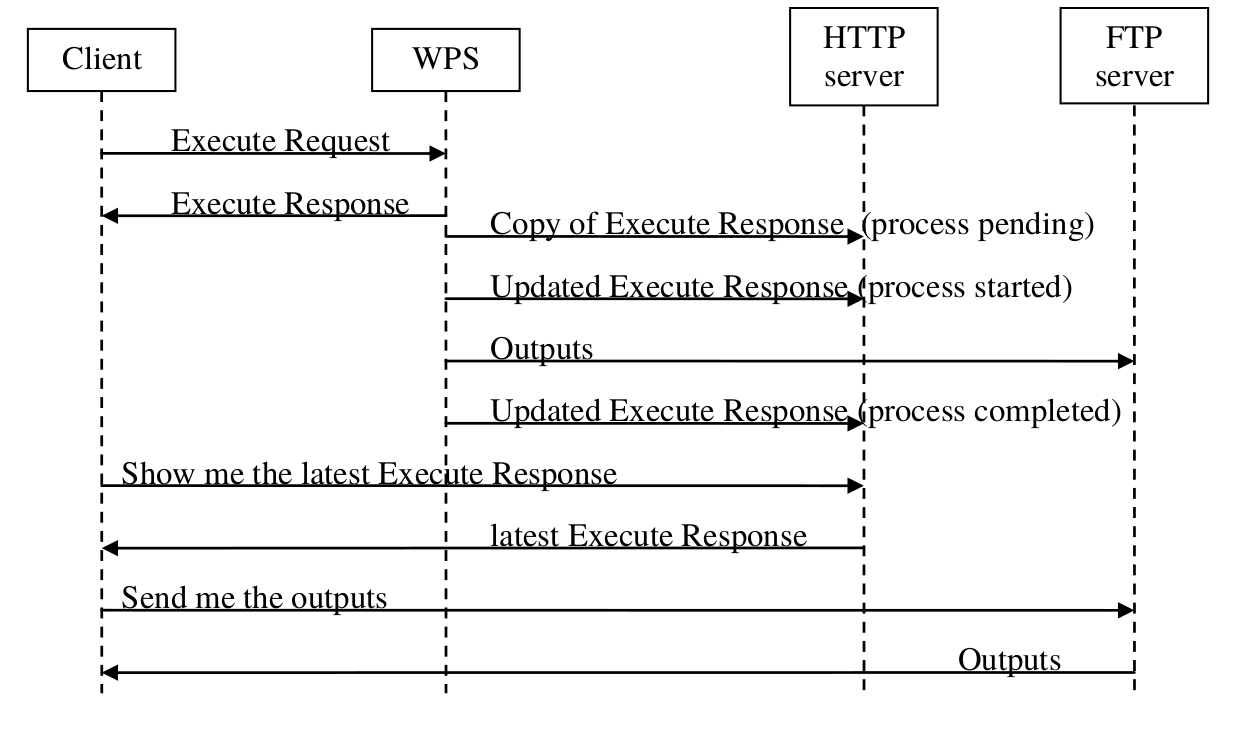
\includegraphics[width=0.9\textwidth]{img/WPS_activity}
\caption{Activity diagram when client requests storage of results, source: \cite{WPS_standart_1.0}}
\label{fig:WPS_activity}
\end{figure}

\paragraph{Execute request}
\begin{table}[h!]
\catcode`\-=12
\centering
\begin{tabular}{|c|c|c|}
\hline
\thead{Name}               & \thead{Optionality} & \thead{Definition and format}    		\\ \hhline{|=|=|=|}
service          	       & Mandatory           & Service type identifier text             \\ \hline
request			           & Mandatory           & Operation name text 				  \\ \hline
version			           & Mandatory           & WPS specification version              \\ \hline
Identifier   	           & Mandatory           & Process identifier \\ \hline
DataInputs		           & Optional            & \makecell{List of inputs provided \\ to this process execution} \\ \hline
ResponseForm	           & Optional            & Response type definition \\ \hline
language   		           & Optional            & Language identifier \\ \hline
\end{tabular}
\caption{Parts of Execute operation request, source: \cite{WPS_standart_1.0}}
\label{tab:WPS_ExecuteRequest}
\end{table}

\paragraph{Execute response}
Ussualy the Execute operation response document is an XML document. Only exception is in case when a response form
of \textit{RawDataOutput} is requested, execution is successful and only one complex output is created, then directly
the produced complex output is returned.

In ussual case response to Execute opetation is an ExecuteResponse XML document. The contents depend on ResponseForm 
request elements.

\begin{table}[h!]
\catcode`\-=12
\centering
\begin{tabular}{|c|c|c|}
\hline
\thead{Name}               & \thead{Optionality} & \thead{Definition and format}    		\\ \hhline{|=|=|=|}
service          	       & Mandatory           & Service type identifier text             \\ \hline
version			           & Mandatory           & WPS specification version              \\ \hline
language   		           & Mandatory           & Language identifier \\ \hline
statusLocation	           & Optional            & \makecell{Reference to location where current\\ExecuteResponse document is stored} \\ \hline
serviceInstance	           & Mandatory           & \makecell{Reference to location where current\\ExecuteResponse document is stored} \\ \hline
Process			           & Mandatory           & Process description \\ \hline
Status			           & Mandatory           & Execution status of the process \\ \hline
DataInputs		           & Optional            & \makecell{List of inputs provided \\ to this process execution} \\ \hline
OutputDefinitions          & Optional            & \makecell{List of definitions of outputs \\desired from executing this process} \\ \hline
ProcessOutputs             & Optional            & \makecell{List of values of outputs \\ from process execution} \\ \hline
\end{tabular}
\caption{Parts of ExecuteResponse data structure, source: \cite{WPS_standart_1.0}}
\label{tab:WPS_ExecuteResponse}
\end{table}

\subsection{WPS implementations}
The OGS WPS is just interface standard that provides rules for standardizing requests and response. It also defines how clients can request
the execution of defined processes and how the outputs are handled. There are several open-source projects that implement this standard 
across the platforms or programming languages.

\begin{itemize}
\item \textit{PyWPS} - Python implementation. This thesis is dedicated to this implementation.
\item \textit{Zoo Project} - WPS implementation written in C, Python and JavaScript.
\item \textit{WPS.NET} - WPS implementation on .NET platform.
\item \textit{52$^{\circ}$North WPS} - Java implementation.
\item \textit{deegree} - Java implementation of many OGC standards including WPS.
\item \textit{WPSint} - Java Spring implementation.
\end{itemize}

\newpage
\section{PyWPS}
PyWPS is server-side implementation of the OGC WPS Standard. It is written in Python. It is currently supporting WPS 1.0.0.
\todo[inline]{Doplnit}

\newpage
\section{Docker}
\paragraph{Containerization} is a lightweight alternative to full machine virtualization. It involves encapsulating an application 
into a container with its own operating environment. It helps to run containerized application on any physical machine without any
worries about dependencies. The origin of containerization lies in the \textit{LinuX Containers {LXC}} format. Containerization
works only in Linux environments and can run only Linux applications.

Docker is not the only one technology for containerization. Other alternatives exist, it is \textit{Kubernets}, \textit{CoreOS rkt}, 
\textit{Open Contrainer Initiative (OCI)}, \textit{Canonical's LXD}, \textit{Apache Mesos and Mesosphere} and many others. 
However Docker is a leader on the field of contanerization and with most public traction is de facto considered as a container standard.
That's why the Docker was choosen for this thesis as a container technology. So from this point on any term \textit{container} refers to
Docker container.

\begin{figure}[h!]
\centering
\begin{floatrow}
\ffigbox{
\includegraphics[width=0.33\textwidth]{img/Docker_kubernetes.png}}{\caption{Kubernetes}}{\label{fig:Dicker_kubernetes}}
\ffigbox{
\includegraphics[width=0.33\textwidth]{img/Docker_rkt.png}}{\caption{CoreOS rkt}}{\label{fig:Docker_rkt}}
\end{floatrow}
\end{figure}

\bigskip

\begin{figure}[h!]
\centering
\begin{floatrow}
\ffigbox{
\includegraphics[width=0.24\textwidth]{img/Docker_lxd.png}}{\caption{Canonical's LXD}}{\label{fig:Docker_lxd}}
\ffigbox{
\includegraphics[width=0.33\textwidth]{img/Docker_mesos.jpg}}{\caption{Apache mesos}}{\label{fig:Docker_mesos}}
\end{floatrow}
\end{figure}

\newpage
\begin{figure}[h!]
\centering

\includegraphics[width=0.6\textwidth]{img/Docker_logo}
\caption{Docker logo}
\label{fig:Docker_logo}
\end{figure}

\paragraph{Docker} is a Linux container technology that allows package and ship applications and everything it needs to execute into a standard
format, and run them on any infractructure.

\begin{figure}[h!]
\centering
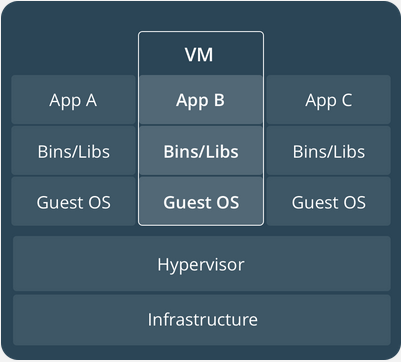
\includegraphics[width=0.6\textwidth]{img/Docker_VM.png}
\caption{Virtual machine architecture, source \cite{Docker_docs}}
\label{fig:Docker_VM}
\end{figure}

\paragraph{Docker container vs. Virtual machine}
Both virtual machines and docker containers are two ways how to deploy multiple, isolated applications on a single platform. They
both offer a way to isolate an application and its dependencies into a self-contained unit that can run anywhere. They both offer
some kind of virtualization. They differ in architecture, see Fig. \ref{fig:Docker_VM}, \ref{fig:Docker_container}.

\noindent
Let's start with virtual machine (Fig. \ref{fig:Docker_VM}) and its layers description from bottom up:
\begin{itemize}
\item \textit{Infrastructure} - It can be a PC, developer's laptop, a physical server in datacenter but as well a virtual private
server in the cloud as Microsoft Azure or Amazon EC2.
\item \textit{Host OS} - Host operating system. In case of native hypervisor this layer is missing. In case of hosted hypervisor
it is probably some distibution of Linux, Windows or MacOS.
\item \textit{Hypervisor} - Also called virtual machine monitor (VMM). It allows to host several different virtual machines
on a single hardware. There are two types of hypervisors:
\begin{itemize}
\item Type 1 -  Also called \textit{bare metal} or \textit{native}. This type is run on the host's hardware to control it as well as manage 
the virtual machines on it. It is much faster and more efficient. This type hypervisors are KVM, Hyper-V or HyperKit.
\item Type 2 - So called \textit{embedded} or \textit{hosted} hypervisors. There hypervisors are run on a host OS as a software. They are slower
and less efficient on the other hand they are much easier to set up. It includes VirtualBox or VMWare Workstation.
\end{itemize}
\item \textit{Guest OS} - Guest operating system. Each VM require own guest operating system which is controlled by hypervisor. Each 
guest OS needs its own CPU and memory resources and starts on hundreds megabytes in size.
\item \textit{Bins/Libs} - Each guest OS needs various binaries and libraries for running the application. It can be \textit{python-dev} or \textit{default-jdk} packages as well as personal packages to run the application.
\item \textit{Application} - The application source code that is desired to be run isolated. Therefore each application or each version of application has to be run inside of its own guest OS with own copy of bins and libs. 
\end{itemize}

\begin{figure}[h!]
\centering
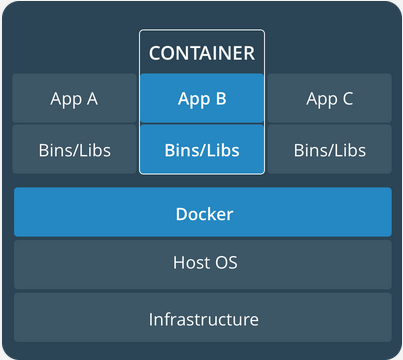
\includegraphics[width=0.6\textwidth]{img/Docker_container}
\caption{Containers architecture, source \cite{Docker_docs}}
\label{fig:Docker_container}
\end{figure}

\noindent
Now, what is different regarding containers (Fig. \ref{fig:Docker_container})
\begin{itemize}
\item \textit{Infrastructure} - PC, laptop, physical or virtual server.
\item \textit{Host OS with container support} - Any OS capable of run Docker. All major distributions of Linux are supported and there are ways
to run Docker even on MacOs and Windows too.
\item \textit{Docker engine} - Also called Docker daemon. It is a service that runs in the beckground on host operating system. It manages all
interaction with containers.
\item \textit{Bins/Libs} - Binaries and libraries required by the application. They get built into special packages called \textit{Docker images}.
The Docker daemon runs those images.
\item \textit{Application} - Each application and its library dependencies get packed into the same Docker image. It is managed independently by the Docker daemon. 
\end{itemize}

\noindent
But the architecture is not the only one difference:
\begin{itemize}
\item Docker use Docker daemon to manage containers, hypervisor manages virtual machines.
\item The Docker daemon communicates directly with host OS and manage resources for each container.
\item VMs usually boot up in minute and more, containers start in seconds.
\item Docker virtualizes operating systems, using VMs is hardware virtualization.
\item VM and container vary in size. VMs start at hundreds of megabytes. Container can be smaller then one megabyte.
\item Containers share the kernel altough they are isolated. VMs are monolitic and stand-alone.
\end{itemize}

\paragraph{Dockerfile}
Dockerfile is a core file that contains instruction to be performed when an image is built. It usually consists from commands to install
packages, calls to other scripts, setting environmental variable, adding files or setting permissions. In Dockerfile there is also defined 
what image is to be used as base image for the build.

\paragraph{Dockerfile instructions}
\begin{itemize}
\item \textit{FROM} - The FROM instruction defines the base image for next instructions and initializes a new build stage. Every Dockerfile
has to start with FROM command. The only exception is ARG command which can be before FROM command.
\item \textit{ARG} - The ARG instruction defines a variable that users can pass at build-time to the builder.
\item \textit{ENV <key>=<value>} - The ENV instruction sets the environment variables. It is key-par value. 
\item \textit{LABEL} - The LABEL instruction adds metadata to an image. A LABEL is a key-value pair. It can be anything from version number to description.
\item \textit{ADD <src> <dest>} - The ADD instruction copies files or directories from source and adds them at the destination path. It also
unzip or untar files when added.
\item \textit{COPY <src> <dest>} - Similar to the ADD instruction it copies files or directories from source and adds them at the destination path. This command doesn't provide any kind of decompression.
\item \textit{RUN <command>} - The RUN instruction will execute any defined command and commit the results.
\item \textit{CMD ["executable","param1","param2"]} - The CMD instruction provides defaults for an executing container. It can include an
executable. In case the executable is ommited the CMD instruction must be used together with the ENTRYPOINT instruction. There can be only
one CMD instruction in Dockerfile. In case there is more CMD the last one will be used.
\item \textit{ENTRYPOINT} - The ENTRYPOINT defines a configuration of container that will run as executable.
\item \textit{WORKDIR /path/to/dir} - The WORKDIR instruction sets the working directory for any RUN, CMD, COPY and ADD instruction that follow
in Dockerfile.
\item \textit{EXPOSE} - The EXPOSE instruction informs Docker that the container listens on the specified network ports at runtime.
\item \textit{VOLUME} - The VOLUME instruction creates a mount point with the specified name and marks it as holding externally mounted volumes from native host or other containers.
\end{itemize}

Except the FROM instruction, all the instructions can be defined from command line when starting docker container. There are more Dockerfile instructions however they are not relevant for this thesis as there are never used in practical part.

\newpage
\begin{lstlisting}[basicstyle=\small,caption={Dockerfile example}]
ARG VERSION=0.9.22
FROM phusion/baseimage:${VERSION}
LABEL maintainer="devs@pywps.example.net"

RUN apt-get update -y && apt-get install -y \
	git \
	python3 \
	python3-dev

RUN git clone https://github.com/geopython/pywps-flask.git
 
WORKDIR /pywps-flask
RUN pip3 install -r requirements.txt

RUN mkdir /etc/service/pywps4
COPY pywps4_service.sh /etc/service/pywps4/run
RUN chmod +x /etc/service/pywps4/run

EXPOSE 5000
ENTRYPOINT ["/usr/bin/python3", "demo.py","-a"]
\end{lstlisting}




\newpage
\part{Practical part}


\newpage
\necislovana{Seznam použitých zkratek}

\begin{tabular}{ll}
\textbf{KVP}& Key Value Pair\\
\textbf{OGC}& Open Geospatial Consortium\\
\textbf{URL}& Uniform Resource Locator\\
\textbf{VM}& Virtual Machine\\
\textbf{VMM}& Virtual Machine Monitor\\
\textbf{WPS}& Web Processing Service\\
\textbf{WMS}& Web Map Service\\
\textbf{WFS}& Web Feature Service\\
\textbf{WCS}& Web Coverage Service\\
\textbf{XML}& eXtensible Markup Language\\
\end{tabular}

\newpage
\begin{thebibliography}{99}
\label{Bibliography}
\bibitem{OGC_news}
Mark Reichardt \textit{OGC Newsletter - October 2004, OGC document number 04-043} [online].
URL: \textless\url{http://www.opengeospatial.org/pressroom/newsletters/200410}\textgreater
\bibitem{WPS_experiment}
Sam Bacharach \textit{OGC announces Web Processing Services Interoperability Experiment} [online].
URL: \textless\url{http://www.opengeospatial.org/pressroom/pressreleases/414}\textgreater

\bibitem{WPS_first}
Open Geospatial Consortium Inc. \textit{OpenGIS ® Web Processing Service, OGC document number 05-007r4, ver. 0.4.0} [online].
URL: \textless\url{https://portal.opengeospatial.org/files/?artifact_id=13149&version=1&format=doc}\textgreater

\bibitem{WPS_standart_1.0}
http://www.opengeospatial.org/pressroom/newsletters/200410

\bibitem{WPS_second}
Open Geospatial Consortium \textit{OGC® WPS 2.0 Interface Standard Corrigendum 1, OGC document number 06-121r3} [online].
URL: \textless\url{https://portal.opengeospatial.org/files/?artifact_id=13149&version=1&format=doc}\textgreater

\bibitem{OGC_common}
Open Geospatial Consortium Inc. \textit{OGC Web Services Common Specification, OGC document number 14-065} [online].
URL: \textless\url{https://portal.opengeospatial.org/files/?artifact_id=20040}\textgreater

\bibitem{Docker_docs}
Docker \textit{Docker documentation} [online].
URL: \textless\url{https://docs.docker.com/}\textgreater

\end{thebibliography}

\end{document}
